\documentclass{article}
\usepackage[utf8]{inputenc}
\usepackage[ngerman]{babel}
\usepackage{enumitem}
\usepackage{graphicx}
\usepackage{amsmath}
\usepackage[version=3]{mhchem} 		%% \ce{CO2} -- automatische subscript der zahlen
\usepackage{booktabs}
\usepackage{subfig}
\usepackage{textcomp}

\begin{document}
\title{Fragen zum Mikrobiologie Tutorium}
\author{Christian Müller \& Ralph Krimmel}

\pagestyle{empty}
\maketitle
\tableofcontents

\pagestyle{headings}
\newpage
\sectionmark{Fragenkatalog 1-3}

\section{Einführung ``Mikrobenparade''}
	\begin{enumerate}
		\item Welches sind die Merkmale des Lebens? Warum sind Prionen keine Lebewesen? Warum können sie trotzdem infektiös sein? \hfill \vspace{4mm}

		Merkmale des Lebens sind zum Beispiel ein Stoffwechsel \& Fortpflanzung.
		Prionen haben keinen eigenen Stoffwechsel,
		die ``chemischen'' Fähigkeiten der Proteine reichen für das Übernehmen von fremden Zellen aus.
		Durch die Übernahme der Zellen sind sie mit ihrem eigenen Erbgut in der Lage,
		sich zu vermehren - deshallb sind sie infektiös.


	\item Nennen Sie mindestens fünf durch Bakterien verursachte Krankheitserreger, die Namen der entsprechenden Bakterien sowie die Bakteriengruppen, denen sie zuzuordnen sind!

		\begin{enumerate}[label=\arabic*)]
			\item \emph{Yersinia pestis} \hfill \\
				Pest, Gammaproteobacteria
			\item \emph{Vibrio cholerae} \hfill \\
				Cholera, Proteobacteria
			\item \emph{Bordetella pertussis} \hfill \\
				Keuchhusten, Proteobacteria
			\item \emph{Mycoplasma pneumoniae} \hfill \\
				Lungenentzündung, Firmicutes
			\item \emph{Bacillus anthracis} \hfill \\
				Milzbrand, Clostridien
		\end{enumerate}


	\item Welche Rolle spielen die Plasmide für die Virulenz von \emph{Bacillus anthracis}?  \hfill \vspace{0.2mm} \\
	
			Die Virulenz von \emph{Bacillus anthracis} ergibt sich
			aus den Plasmiden ``px01'' und ``px02''.
			Im ersten Plasmid (``px01'') wir ein potentes Toxin codiert,
			das zweite Plasmid (``px02'') ist für die Bildung einer Kapsel verantwortlich.
			Durch die Kapsel wird die Phagocytose der Zelle verhindert,
			wodurch das Toxin wirken kann.


		\item Nennen Sie einige Bakterien, die für die Landwirtschaft/unsere Ernährung von entscheidender Bedeutung sind. \hfill \\
		
		\emph{Saccharomyces cerevisae}, die Bier- \& Bäckerhefe,
		ist ein wichtiger Teil der Nahrungsmittelproduktion.
		\emph{Lactobacillus casei} ermöglicht die zum Beispiel die Herstellung von Sauerkraut,
		und das Haltbarmachen von Milchprodukten.
		Diverse Arten von \emph{Rhizobium} ermögliche die Fixierung von molekularen Stickstoff,
		den sie den Wurzeln von Pflanzen bereitstellen.
		Diese, sogenannten ``Knölchenbakterien'', sind Grundlesgen für die Stickstoffversorgung der Pflanzen.
	\end{enumerate}

\section{Geschichte der Mikrobiologie}
	\begin{enumerate}
		\item Womit beschäftigen sich die Koch’schen Postulate?
		Bei welcher Gelegenheit wurden Sie von Robert Koch aufgestellt und was besagen sie? \hfill \vspace{4mm}
	
		\begin{enumerate}[label=\arabic*)]
			\item In einem Infizierten Organismus müssen Erreger nachweisbar sein.
			\item Die offenbaren Errger müssen in reiner form isoliert werden.
			\item Mit den Reinkulturen müssen gesunde Organismen identifiuert werden können.
		\end{enumerate}
		Sie wurden von Robert Koch während der Entdeckung von \emph{Bacillus anthracis},
		dem Erreger des Milzbrandes aufgestellt,
		um zu Ermitteln ob die Bakterien Folge oder Ursache der Krankheit sind.	
		

		\item In einem klassischen Experiment konnte Griffith 1928 einen apathogenen Stamm von
		\emph{Streptococcus pneumoniae} in einen pathogenen Stamm umwandeln.\\
		Wie funktionierte dieses Experiment? Worauf beruht es? 
		Welche bahnbrechende Schlußfolgerung wurde daraus gezogen? \hfill \vspace{4mm}
		
		\begin{figure}[ht!]
		\leavevmode
		\begin{center}
		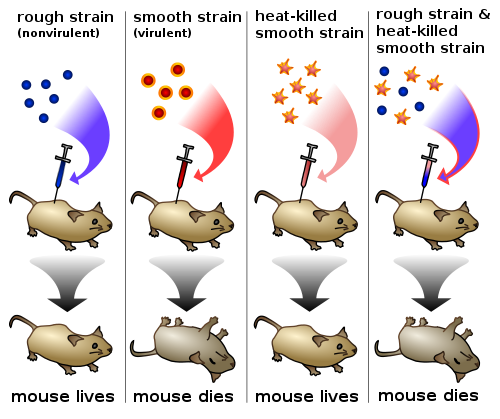
\includegraphics[scale=0.47]{./pictures/griffith_exp_500}
		\end{center}
		\caption{\slshape{Griffith's Experiment.}}
		\label{fig:griffith}
		\end{figure}

		Es gibt zwei Zelltypen von \emph{Streptococcus pneumoniae} der ``s''-Typ
		bildet eine Kapsel aus, und erscheint deshalb im Lichtmikroskop glatt (``smooth').
		Der \& ``r''-Typ, kann keine Kapsel ausbilden und erscheint im lichtmikroskopischen Bild
		mit einer rauen (``rough'') Oberflächen.
		Nur Zellen des ``s''-Typs lösen in Mäusen Lungenentzündung aus,
		die Zellen des ``r''-Typs sind sind nicht durch eine Kapsel geschützt und können
		vom Immunsystem erkannt und bekämpft werden.

		Grifith tötet, in dem nach ihm benannten Experiment,
		Bakterien des ``s''-Typs durch erhitzen ab.
		Werden einer Maus nur abgetötete Erreger des ``s''-Typs injeziert,
		bleibt dieses gesund.
		Werden sowohl abgetöte Bakterien des ``s''-Typs,
		als auch lebenden Bakterien des ``r''-Typs injeziert,
		erkrankt die Maus an einer Lungenentzündung.
		In der Maus befinden sich dann Zellen vom \emph{Streptococcus pneumoniae} 
		die eine Kapsel ausbilden.

		Griffith hat gezeigt, dass die Fähigkeit zur Kapselbildung von den toten ``s''-Zellen
		auf die lebenden ``r-''Zellen übertragen worden war.
		1944 wurde von Oswald Avery gezeigt,
		dass diese Transformation auf einer Übertragung von DNS beruhte.


		\item Mycoplasmen sind die wichtigsten Objekte der synthetischen Biologie. 
		Nennen Sie einige Eigenschaften dieser Bakterien,
		die sie für die Forschung allgemein und die synthetische Biologie im besonderen interessant machen. \hfill \vspace{4mm}

		Da die Mycoplasmen eines der kleinsten Genome besitzen sind sie besonderst für die synthetische Biologie interessant.
		Das Genom von \emph{Mycoplasma pneumoniae},
		dem Errreger der Pneumonie,
		umfasst beispielsweise nur 816 kBp mit 688 Genen.
		Regulation findet kaum statt.
		Bei \emph{Mycoplasma pneumoniae} handelt es sich um ein gram-positives Bakterium ohne Zellwand.
		Es haftet an, und bweget sich dann gleitend fort.
		Auch die nahe Verwandten von \emph{Mycoplasma pneumoniae},
		haben kleine Genome und sind meist pathogen.

		An ihnen lässt sich gut erkennen,
		welche Stoffwechsel funktionen für ``Leben'' obligat sind.
		Ein minimales Gen-Set lässt sich ermitteln und künstlich erzeugen.

	\end{enumerate}


\newpage
\sectionmark{Cytologie}

\section{Cytologie}
\label{sec:cytologie}
	\begin{enumerate}
		\item Wie funktioniert in Grundzügen ein Fluoreszenzmikroskop? Welche Unterschiede bestehen zur konventionellen Lichtmikroskopie?				
			Mit Licht in bestimmten Wellenlängen werden Stoffe
			oder auch Proteine (z.B. ``GFP'') im Objekt zum	fluoreszieren angeregt.
			So können bestimmte Strukturen sichtbar gemacht werden.
			Bei der Lichtmikroskopie wird das Objekt mit einem Spektrum des sichtbaren Lichtes
			beleuchtet.

		\item\label{tab:quest_cyt_resolution} Wie hoch ist die Auflösung eines Lichtmikroskops?
			Kennen Sie eine Formel zur Berechnung der Aufösung (vgl. Mikrobiologisches Grundpraktikum)?

		Die Auflösung eines Lichtmikroskops ist Abhängig von der Wellenlänge des Lichtes.
		Diese liegt bei grünem Licht bei 550 nm und begrenzt die die optische Auflösung.
		Die nummerische Apertur liegt bei der Verwendung von Immersionsöl bei etwa 1,3.
		Somit ist der kleinste Abstand zweier Bildpunkte bei einem 100-fach Objektiv:

		\begin{center}
		\begin{math}
			d_{0} = \dfrac{100}{1,30} = 0,3 \hspace{27mm} |\hspace{3mm} \lambda = 550 nm
		\end{math}
		\end{center}

		\item Wie wirkt sich die Größe eines Organismus auf die Stoffwechselleistungen aus? Warum?
			
			Das Verhältnis von Oberfläche durch Volumen eines (kugelförmigen) Organismus,
			nimmt mit zunehmendem Radius ab.
			Dies wird mit der Oberflächenregel beschrieben, welche durch Max Rubner anhand von Säugetieren ermittelt wurde.
			Sie besagt, dass die spezifische Stoffwechselrate für (Stoffverbrauch/kg Körpergewicht)
			mit abnehmender Körpergröße ansteigt.

			Die Oberflächenregel lässt sich auch auf Mikroorganismen übertragen.
			Hier wird der Transport des Substrates über die Membran ins Cytosol zum limitierende Faktor.
			Eine Optimierung wird hier duch geringe Zellgröße und hohe Teilungsrate erreicht.
			Auch spezielle Wuchsformen wie zum Beispiel Stäbchen
			oder Fillamente und andere Zellanhängsel vergrößern die Membranfläche.

		\item Stellen Sie die Eigenschaften von Eu- und Prokaryoten einander gegenüber. Welche Eigenschaften (die Prokaryoten nicht haben) ermöglichen es Eukaryoten, große Zellen zu bilden? Warum sind dennoch einige Prokaryoten groß?

			Der Namensgebende Unterschied bezieht sich auf das Vorhandensein eines echten Zellkerns (Nucleus) bei dem Eukaryoten.
			Dieser Zellkern schließt durch eine Doppel-Lipidmembran die DNA ein
			und dient als Raum für die Transkription der DNA in mRNA.

			Bei einere prokayrotische Zelle wie in Abbildung \ref{fig:prokarya} dargestellt,
			ist somit kein Zellkern vorhanden.
			Die DNA liegt verpackt im Cytosol,
			wo auch die vollständige Proteinbiosynthese stattfindet.
			Die Verpackung der DNA geschieht jedoch im Gegensatz zu den Eukaryoten ohne Histone.
			Zusätzlich haben einige Bakterien noch ringförmige oder lineare Plasmide,
			welche als zusätzliche Träger Genmaterial dienen.
			
			\begin{figure}[ht!]
			\leavevmode
			\begin{center}
			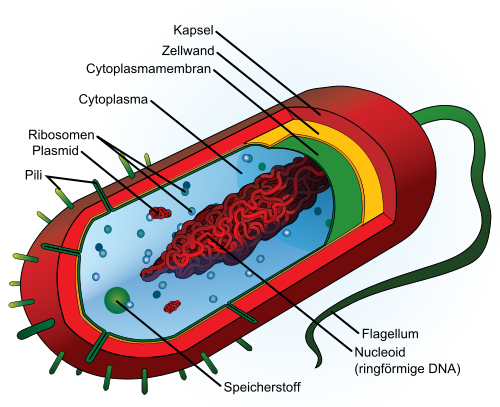
\includegraphics[scale=0.47]{./pictures/avg_prokaryote_cell_500}
			\end{center}
			\caption{\slshape{Typische prokaryotische Zelle.}}
			\label{fig:prokarya}
			\end{figure}
	
			Die Translation findet bei Prokyoten mit 70 S Ribosomen statt,
			welche frei im Cytosol vorliegen.
			Prokaryoten besitzen keine membranbegrenzten Organellen wie zum Beispiel Mitochondrien oder Vakuolen.

			\begin{figure}[ht!]
			\leavevmode
			\begin{center}
			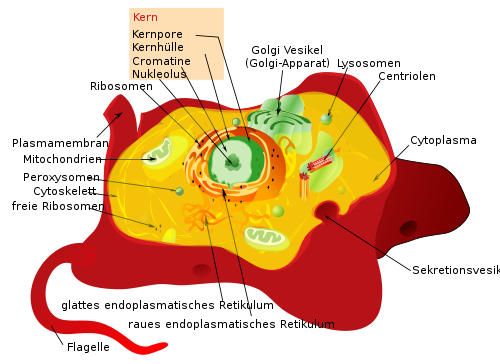
\includegraphics[scale=0.47]{./pictures/animal_cell_500}
			\end{center}
			\caption{\slshape{Tierische Zelle als Beispiel einer eukaryotischen Zelle.}}
			\label{fig:eukarya}
			\end{figure}

			Die reife mRNA wird bei Eukaryoten mit 80 S Ribosomen translatiert.
			Diese befinden sich am rauen endoplasmatischen Retikulum,
			welches bei Prokaryoten nicht vorhanden ist.
			Beispielaft für eukaryotische Zellen ist die in Abbildung \ref{fig:eukarya} dargestellte,
			tierische Zelle.

			Eukaryotische Zellen haben Transportsysteme die den Transport von Stoffen im Cytosol ermöglichen.
			Durch das Fehlen von Vakuolen in prokaryotischen Zellen sind diese in ihrer größe Beschränkt.
			Die größten Bekannten Zellen hat der \emph{Epulopiscium fishelsoni} welcher mit den Clostriedien verwandt ist.
			Seine polyploiden Zellen können über 0,5 cm groß werden,
			und maximiert so seine Oberfläche.
			
			Siehe dazu auch Frage \ref{tab:quest_cyt_resolution} in Kapitel \ref{sec:cytologie}. 

		\item Wie klein kann ein autonom lebender Prokaryot werden? Begründen Sie Ihre Abschätzung.
			
			Die kleinsten Prokaryoten mit einem Volumen von weniger als \begin{math}0,1\ \mu m^{3}\end{math} sind weit verbreitet
			in marinen Ökosystemen.
			Auch obligat symbiontische oder pathogene Bakterien können durch Reduktion ihres Zellinventares diese geringen Größen erreichen.
			Zellen mit weniger als \begin{math}0,2\ \mu m - 0,3\ \mu m\end{math} wären nicht lebensfähig,
			da zumindest Ribosomen, essentielle Metabolite sowie DNA und Proteine untergebracht werden müssen.

		\item Was sind Einheitsmembranen (unit membranes)? Wo finden sie sich in der prokaryotischen Zelle?

			Einheitsmembranen bestehen aus einer Doppelschicht von amphiphilen Fettsäuren.
			Das heisst, die Fettsäuren bestehen aus einem hydrophphilen Kopf und einem hydrophoben Schwanz.
			Bei passenden Verhältnis von Wasser zu Lipid, bildet sich spontan eine Doppelschicht der amphiphilen Fettsäuren.
			Hierbei stehen die hyprophoben Schwänze auf einander.
			Die Lipid-Doppelmembran ist etwa 5 nm dick.
		
			Die Köpfe bestehen meistens aus Phospholipiden,
			wobei am Glycerin zwei Kohlenwasserstoffketten,
			mit typischerweise zwischen 14 und 24 Kohlenstoffatomen,
			gebunden sind.
			Während eine der beiden Kohlenstoffketten meist gesättigt ist,
			hat die andere einen oder mehre \textit{cis}-Doppelbindungen.
			Diese ungesättigeten Fettsäuren führen zu einer entsprechenden Anzahl von ``Knicken'' in der Kette,
			welche die Fluidität der Membran beeinflussen.
			Die Fluidität der Membran wird durch ihre Zusammensetzung bestimmt.
			So sind weitere Einflussgrößen die Temperatur und
			die Anzahl der enthaltenen Proteine.

			Die wesentlichen Funktionen von Biomembranen sind:

			\begin{itemize}
				\item \emph{Permeabilitätsbarriere} \hfill \\
				Selektive Barriere für den Transport ins Cytosol oder aus diesem hinnaus.
				\item\emph{Proteinverankerung} \hfill \\
				Membranständigproteine zur gezielt Synthese von Stoffen in deffinierte Kompartimente.
				\item\emph{Energiekonservierung} \hfill \\
				Aufbau und Verbrauch von protonenmotorischen Kräften entlang der Membran.
			\end{itemize}

			\begin{figure}[ht!]
			\leavevmode
			\begin{center}
			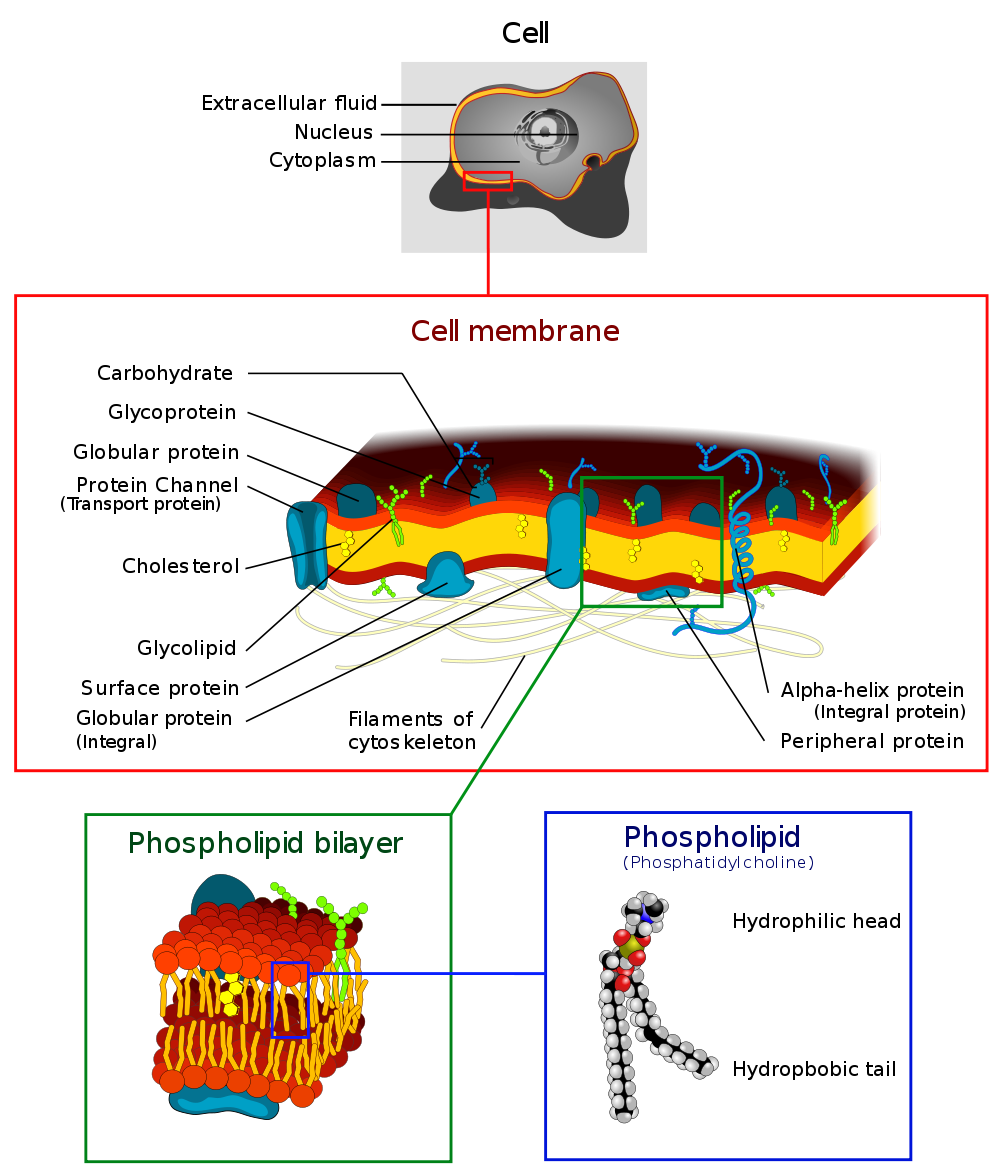
\includegraphics[scale=0.34]{./pictures/cell_membrane_diag_1000}
			\end{center}
			\caption{\slshape{Lage und Aufbau von Zellmembran.}}
			\label{fig:cellmembrane}
			\end{figure}

		\item Wie können Membranen modifiziert werden, um sie unterschiedlichen Umgebungstemperaturen anzupassen?
			
			Da die Umgebungstemperatur entscheident für die Membranfluidität ist,
			gibt es verschiedene Möglichkeiten um Membranen an diese anzupassen.
			Besonders wichtig ist der Anteil der ungsättigeten Fettsäuren.

			Bestehen die hydrophoben Schwänze aus gesättigenten Fettsäuren,
			ist wenig Bewegung in der Membran möglich die Phospholipide nahe beieinander liegen.
			Durch ungsättigte Fettsäuren sind die abständer der einzelnen Phospholipid-Moleküle weiter auseinander,
			da die ``Knicke'' Freiräume schaffen.
			Zusätzlich können Moleküle wie \emph{Cholesterin} (Eukarya) oder \emph{Hopanoide} (Prokarya) in die Membran eingelagert werden.
			Diese Moleküle sind sowohl funktionell als strukturell sehr ähnlich.
			Sie erhöhen den Abstand der Phospholipide,
			und reduzieren wiederum die Viskosität. %% korrekt?
			Die Anzahl der in der Membran gebundenen Proteine hat auch Einfluss auf die Membranfluidität.

		\item Welche Proteine finden Sie typischerweise in Membranen? Welche Funktionen habe sie? Was sind Hopanoide?
			
			In Membranen befinden sich vorallem Transportproteinen.
			Diese ermöglichen den gesteuerten Transport von Stoffen durch die Membran.
			Dabei gibt es drei Transportvarianten:
			\begin{enumerate}[label=\arabic*)]
				\item \emph{Einfacher Transport} \hfill \\ 
					Getrieben durch die protonenmotorische Kraft.
				\item \emph{Gruppentranslokation} \hfill \\ 
					Chemische Veränderung der transportierten Verbindung,
					getrieben durch Phospoenopyruvat.
				\item \emph{ABC-System} \hfill \\ 
					Mit Transportproteinen unter ATP-Verbrauch.
			\end{enumerate}

			tbc.

		\item Stellen Sie vergleichend die unterschiedlichen Zellwand-Typen von verschiedenen Bacteria und Archaea gegenüber.
		\item Wie ist die Äußere Membran (outer membrane) von Bakterien wie z.B. \emph{Escherichia coli} gebaut?
		\item Worauf beruht die Festigkeit der Peptidoglycanstruktur? 
			Die Peptidoglycanschicht is der der Cytoplasmamembran aufgelagert.
			Diese beiden Schichten werden mit Lipoteichonsäuren verbunden.
			In Gram-positiven Bakterien wird die Peptidoglycanschicht 20-80 nm dick,
			in Gram-negative erreicht sie maximal 10 nm.

			Die Peptidoglycanschicht baut sich aus durchgehenden Polyscharidketten auf,
			welche sich welchselnder Folge von N-Acetyglucosamin und N-Acetylmuraminsäure zusammensetzen.
			Die Quervernetzung dieser Ketten wird von Peptidbrücken erzeugt,
			wobei auch D-Aminosäuren verwendet werden.
			Durch diese Quervernetzung,
			des auch als Murein bezeichneten Komplexes,
			wird die mechanische Stabilität erreicht.


		\item Auf welchem Prinzip beruht die Gram-Färbung? Können Sie mit der Färbung sicher die unterschiedlichen Typen von Zellwänden unterscheiden?
			Anhand der Gramfärbung lassen sich Zellwandtypen im Prinzip nicht unterscheiden.
			Jedoch wird ein positives Ergebniss der Gramfärbung (Gram-positiv),
			mit dem Zellwandtyp der \emph{Firmicutes} und der \emph{Actinobacteria} gleichgesetzt.
			Wohingegen der Zellwandtyp der \emph{Proteobacteria} als Gram-negativ bezeichnet wird.

			Bei der Gramfäbung wird ermittelt ob ein Farblack nach dem Einbringen in die Zelle wieder herrausgewaschen werden kann,
			oder nicht.
	\end{enumerate}


\newpage
\sectionmark{Gärung I}

\section{Gärung I}
\begin{enumerate}
	\item Was versteht man unter einer klassischen Gärung und wie unterscheidet sie sich von Atmungsprozessen?
	
		Als Gärung bezeichnet man eine intern ausbalancieten Oxidations-Reduktion.
		Die klassischen Charakteristiken einer Gärung sind:
		\begin{itemize}
			\item keine externen e\textsuperscript{-}-Akzeptoren
			\item keine direkte mit Substratoxidation gekoppelte Elektronentransport-Phosphorylierung.
			\item organische Verbindungen als Substrate
		\end{itemize}

	\item Benennen Sie Gärungsprodukte und Organismen, die diese Produkte produzieren.
		
		In Tabelle \ref{tab:gaerungsprodukte} sind einige Organismen und ihre Gärungsprodukte aufgeführt.
		Zentralles Intermediat ist in den aufgeführten Vorgängen immer Pyruvat.
		\begin{table}[h!]
		\begin{center}
		\begin{tabular}{l l} 
		\toprule
			Organismengruppe			&	Gärungsprodukt\\
			\midrule
			Milchsäurebakterien		&	Lactat\\
			Hefen							&	Ethanol\\
			Propionibakterien			&	Propionat\\
			Coli-Aerogenes-Gruppe	&	Butandiol\\
			Clostridien					&	2-Propanol, Butanol\\
		\bottomrule
		\end{tabular}
		\caption{Verschiedenen Mikroorganismen und ihre Gärungsprodukte.}
		\label{tab:gaerungsprodukte}
		\end{center}
		\end{table}

	\item Wieso muss bei einer Gärung die Wasserstoffbilanz ausgeglichen werden?
	\item Auf welchen Wegen kann der initiale Glucoseabbau bei unterschiedlichen Gärungen erfolgen (mit Beispielen)?
	\item Geben Sie Beispiele für C-Quellen, die von Saccharomyces fermentiert, veratmet, bzw. nicht verwertet werden können.

	Glucose (\ce{C6H12O6}) kann sowohl veratmet als auch vergärt werden.	
		\begin{description}
			\item[Atmung] \hfill\\
				\ce{C6H12O6} + \ce{602} \textrightarrow \ \ce{6CO2} + \ce{6H2O} \hfill 32-36 ATP	
			\item[Gärung] \hfill\\
				\ce{C6H12O6} \textrightarrow \ \ce{2CO2} + 2\ce{CH3}-\ce{CH2}-\ce{OH} \hfill 2 ATP
		\end{description}

	\item Welche Enzyme werden für die Alkoholische Gärung benötigt und welches ist das Schlüsselenzym?

		Für die Alkoholische Gärung werden sowohl im Embden-Meyerhof-Parnas-Weg,
		als auch im Entner-Doudoroff-Weg folgende Enzyme benötigt:
		\begin{itemize}
			\item Pyruvat-Decaboxylase
			\item Ethanol-Dehydrogenas
		\end{itemize}
		
	\item Bei welchen Schritten werden bei der Alkoholischen Gärung ATP gebildet oder Reduktionsäquivalente verbraucht?
	\item Wie und warum unterscheidet sich die ATP-Ausbeute bei den alkoholischen Gärungen von Zymomonas mobilis und Saccharomyces cerevisiae?
	\item Welche Standorte besiedeln Milchsäurebakterien?
		
		Milchsäurebakterien finden sich in folgenden Habitaten:
		\begin{itemize}
			\item Pflanzen
			\item Milch, Milchprodukte
			\item Darm
			\item Schleimhäute
			\item Hautflora
		\end{itemize}

	\item Im Rahmen welcher Gärung taucht Methylmalonyl-CoA als Zwischenprodukt auf?
	\item Was ist das Schlüsselenzym der Milchsäuregärung?

		Kandidaten:
		\begin{itemize}
			\item Laktat-Dehydrogenase
			\item Phosphoketolasee
		\end{itemize}

	\item Benennen Sie Charakteristika von Bifidobakterien?
		
		Der Name der ergibts sich aus ihrer ``gespaltenen'', V- bzw. Y-Form.
		Ihr Habitat ist die Darmflora von Säuglingen,
		wohin sie durch die Muttermilch gelangen.
		In Kuhmilch sind sie jedoch nicht vorhanden.
		Es handelt sich um nicht aerotolerante Bakterien,
		die eine \ce{CO2} Atmosphäre benötigen.
		Bifidobakterien gären über den Phosphoketolase-Nebenweg.

	\item Wo verzweigen sich die Wege der homo- und der heterofermentativen Milchsäuregärung?
	\item Wie kommen die Löcher in den Emmentaler Käse?

		Die Löcher entstehen durch die \emph{Propionibakterien}.
		Sie vergären das Laktat auch zu \ce{CO2} (s.u.),
		welches die Löcher bedingt.
		\emph{Propionibakterien} sind gram-positive und	aerotolerant.
		Sie besiedeln den Pansen und Darm von Wiederkäuern und bauen Glukose über den
		Fruktose-1,6-bisphosphat-Weg ab, die weiter Gärung erfolgt mit:
		
		3 Laktat \textrightarrow \ 2 Propionat + 1 Acetat + \ce{CO2} + \ce{H2O}

	\item Nennen Sie Arten der Enterobacteriaceae.
	\item Welches Verhältnis haben Enterobacteriaceae zum Sauerstoff?
	\item Welche Gärprodukte werden von Enterobakterien gebildet?
	\item Welche zwei Gärungstypen werden bei der gemischten Säuregärung unterschieden?
	\item Benennen sie hierfür repräsentative Vertreter
	\item Wie entstehen bei der gemischten Säuregärung Formiat, Wasserstoff und Kohlendioxid?
	\item Wie entsteht 2,3-Butandiol? und welche Enterobakterien produzieren es?
	\item Unter welchen Bedingungen wird die Bildung von 2,3-Butandiol begünstigt?
	\item Wie verteilen sich die Produkte bei der Vergärung von Glucose durch Escherichia coli bei Wachstum unter alkalischen bzw. sauren Bedingungen?
	\item Wie entsteht Succinat bei anaeroben Wachstum von Escherichia coli? Handelt es sich um einen Atmungs- oder Gärungsprozess?
\end{enumerate}

\newpage
\sectionmark{Gärung II}

\section{Gärung II}
\begin{enumerate}
	\item Was für eine Reaktion katalysiert die Phosphoketolase und für welchen Typ von Milchsäurebakterien ist sie bedeutsam?

		Die Phosphoketolase kataklysiert die heterofermentative Milchsäuregärung.
		Dieser Typ der Gärung wird von Bifidobakterien verwendet-
		Sie sind nicht aerotolerant und benötigen eine \ce{CO2}-Atmosphäre.
		Die heterofermentative Milchsäuregärung (Pentose-P-Weg= wird auch durch geführt von \emph{Leuconostoc} und
		\emph{Lactobacillus brevis}.
		
	\item Wobei und welche schädlichen reaktiven Sauerstoffverbindungen können entstehen?

		\begin{description}
			\item[Superoxid \ce{O2-}] \hfill\\
				Superoxid-Dismutase
			\item[Wasserstoffperoxid \ce{H2O2}] \hfill\\
				Katalase
			\item[Hydroxyl-Radikal \ce{OH-}] \hfill\\
		\end{description}

	\item Nennen sie Beispiele für Entgiftungsmechanismen.
		
			s.o.

	\item Nennen sie charakteristische Eigenschaften von Clostridien.
		
		Die Clostrieden spalten sich auf in die Gruppe der Saccharolytischen Clostrieden,
		welche Zucker verstoffwechseln und
		in die Peptolytischen Clostriedien,
		welche Aminosäuren verstoffwechseln.
		Beiden Gruppen sind folgende Eigenschaften gemein:
		\begin{itemize}
			\item Stäbchenform
			\item Gram-positiv
			\item niediger GC-Gehalt des Genoms
			\item strikt anaerob
			\item Sporenbildner
			\item bevorzugen neutralen oder alkalischen pH
			\item z.T. \ce{N2}-Fixierer
		\end{itemize}

	\item Welche Substrate können saccharolytische bzw. peptolytische Clostridien verwerten?

		\begin{description}
			\item[Saccharolytische Clostridien] \hfill \\
				Cellulose, Zucker, Stärke, Pectin
			\item[Peptolytische Clostridien] \hfill \\
				Aminosäuren
		\end{description}

	\item Welche Gärprodukte können aus Glukose gebildet werden?
		
		Glukose kann von Clostriedien zu Folgenden Substanzen fermentiert werden:
		\begin{itemize}
			\item Acetat
			\item Aceton
			\item Butanol
			\item Butyrat
			\item \ce{CO2}, \ce{H2}
			\item Ethanol
			\item Propionat
			\item Succinat
		\end{itemize}

	\item Welches charakteristisches Enzym ist bei den Clostridien für die Pyruvatspaltung verantwortlich?

		Pyruvat-Ferredoxin Oxidoreduktase.

	\item Welchen Vorteil bringt den Clostridien die \ce{H2}-Entwicklung?

		%TODO

	\item In welchen Reaktionen kann bei Clostridien durch Substratkettenphosphorylierung ATP gebildet werden?

		Bei der Umsetzung von Butyryl-CoA mit der Butyrat-Kinase zu Butyrat und
		bei der Umsetzung von Acetyl~P zu Acetat durch die Acetat-Kinase

	\item Durch welche Milieubedingungen wird die Bildung von Aceton bzw. Butanol durch Clostridium acetobutylicum begünstigt?

		Die Bildung von Aceton und Butanol findet bevorzugt bei leicht sauren pH-Werten statt.
		% wenn richtig interpretiert Gaerung2 S.11 

	\item Welcher Zelldifferenzierungsprozess ist mit der Lösungsmittelbildung gekoppelt?
		
		Der Beginn der Sporenbildung ist mit der Bildung von Butanol, Aceton und Ethanol assoziert.

	\item Welche Umstände begrenzen die biotechnologische Produktion von Lösungsmitteln aus Glucose durch \emph{Clostridium acetobutylicum}?
			
		Butanol ist toxisch für \emph{Clostridium acetobutylicum} und
		begrenzt somit die Konzentration auf etwa 20 g/l.
		Zusätzlich ist auf Grund der Stoffwechselwege 
		der Ertrag auf maximal 30 kg Lösungsmittel pro 100 kg Substrat begrenzt.
		
	\item Nennen Sie pathogene Clostridienarten und die pathogene Wirkung.
		
		\begin{table}[h!]
		\begin{center}
		\begin{tabular}{p{2.399cm} p{3.4cm} p{5.0cm}} 
		\toprule
		Art	&	Verantwortlichkeit	&	Symptome\\
		\midrule
		\emph{C. histolyticum},	\emph{C. septicum}	&	Wundinfektion				&	Wachstum in tiefen Wunde, übelriechend \\
		\emph{C. tetani}				&	Wundstarrkrampf			&	Tetanus-Toxin: blockiert Neurotransmitterausschüttung  an inhibitorischen Synapsen \\
		\emph{C. botulinum}			&	Lebensmittelvergiftung, Botulismus	&	Tetanus-Toxin: blockiert Neurotransmitterausschüttung an Synapsen der stimulatorischen Neuronen an Muskeln \\
		\emph{C. butyricum}, \emph{C. sporogenes}			&	Lebensmittelverderb		&	Verderb unzureichen haltbargemacher Lebensmittel, Explodierende-Konserven\\
		\bottomrule
		\end{tabular}
		\caption{Verschiedene pathogene Clostriedien und die von ihen Erzeugten Krankheiten.}
		\label{tab:pathClostridien}
		\end{center}
		\end{table}

	\item Was versteht man unter der Stickland-Reaktion? Nennen sie ein Beispiel für diese Reaktion.
		
		Die Stickland-Reaktion ist die paarweise Vergärung von Aminosäuren.
		Es handelt sich hierbei um eine Redox-Reaktion bei der eine Aminosäure oxidiert,
		die andere reduziert wird.
		Die Produkte einer solchen Reaktion sind iummer \ce{NH3}, \ce{CO2} und 
		eine Carbonsäure mit einem C-Atom weniger als die oxidierte Aminosäure.

		In Tabelle \ref{tab:stickland} befindet sich eine Aufstellung von möglichen Aminsäurepaaren.
		
		\begin{table}[h!]
		\begin{center}
		\begin{tabular}{l l} 
		\toprule
		oxidierte Aminosäure	&	reduzierte Aminosäure	\\
		\midrule
		Alanin		&	Glycin			\\
		Leucin		&	Proline			\\
		Isoleucin	&	Hydroxyprolin	\\
		Valin			&	Tryptophan		\\
		Histidin		&	Argenin			\\
		\bottomrule
		\end{tabular}
		\caption{Paare von Aminosäuren die eine Stickland-Reaktion durchlaufen können.}
		\label{tab:stickland}
		\end{center}
		\end{table}

	\item Wie kann Ethanol vergärt werden?
		
		Ethanol kann mit Wasser zu Acetat und Wasserstoff fermentieren.
		
		\ce{2CH3CH2OH} + \ce{2H2O} \textrightarrow \ce{4H2} + \ce{2CH3COO-} + \ce{2H+}
\end{enumerate}

\newpage
\sectionmark{Wachstum der Bakterien I}

\section{Wachstum der Bakterien I}
\begin{enumerate}
	\item Nennen Sie fünf Makroelemente, die alle Organismen zum Leben brauchen und deren Quellen für Bakterien (dabei sollte mindestens 1 Metall sein)!

		Einige, für Mikroorganismen wichtige Markoelemente und ihre Quellen sind in Tabelle \ref{tab:makroelemente}
		beschrieben.
		\begin{table}[h!]
		\begin{center}
		\begin{tabular}{l l} 
		\toprule
		Element	&	Bereitstellung	in der Natur \\
		\midrule
		C			&	\ce{CO2}, organische Stoffe \\
		H			&	\ce{H2O}, organische Stoffe \\
		O			&	\ce{H2O}, \ce{O2}, organische Stoffe \\
		N			&	\ce{NH3}, \ce{NO3-}, \ce{N2}, organische Stoffe \\
		P			&	Phosphat \\
		S			&	\ce{H2S}, organische Stoffe, Sulfide \\
		\midrule
		K			&	Kaliumsalze \\
		Mg			&	Magnesiumsalze \\
		Na			&	\ce{NaCl}, Natriumsalze \\
		Ca			&	Salze \\
		\midrule
		Fe			&	\ce{FeS}, Eisensalze \\
		\bottomrule
		\end{tabular}
		\caption{Mikroelementen und ihre Quellen für Mikroorganismen}
		\label{tab:makroelemente}
		\end{center}
		\end{table}

	\item Nennen Sie einige Mikroelemente und erklären Sie, wofür diese Elemente benötigt werden!
	
		Einige, für Mikroorganismen wichtige Mirkoelemente und ihre Funktionsort sind in Tabelle \ref{tab:mikroelemente}
		beschrieben.
		\begin{table}[h!]
		\begin{center}
		\begin{tabular}{l l} 
		\toprule
			Element	&	Funktion in der Zelle \\
			\midrule
			Co			&	\ce{B12}, Transcaboxylase \\
			Cu			&	Atmung, CytC-Oxidase, Photosynthese\\
			Mn			&	Photosystem II, Superoxiddismutase \\
			Mo			&	Nitrogenase, Nitratreduktase, Formiat-DHG \\
			Ni			&	Hydorgenase, Co-F430 (Methanogene), \ce{CO}-Dehydrogenase \\
			Se			&	Formiat-DHG, Hydrogenase\\
			W			&	Formiat-DHG \\
			V			&	Vanadium-Nitrogenase \\
			Zn			&	Alkohol-DHG, RNA-/DNA-Polymerase \\
			Fe			&	Cytochrome, Katalasen, FeS-Proteine, alle Nitrogenasen \\
		\bottomrule
		\end{tabular}
		\caption{Mikroelementen und ihre Quellen für Mikroorganismen}
		\label{tab:mikroelemente}
		\end{center}
		\end{table}

	\item Stellen Sie sich vor, sie kultivieren \emph{E. coli}! Sie starten eine Kultur mit 3000 Zellen und kultivieren sie dann unter optimalen Bedingungen für 12 Stunden. Zeichnen Sie schematisch die Wachstumskurve dieser Kultur (bitte denken Sie an die Achsenbeschriftung und die Skalierung)!

		In Abbildung \ref{fig:ecoliplot} ist die Anzahl der Zellen von \emph{E. coli} innerhalb der ersten 12 Stunden aufgetragen.	
		\begin{figure}[ht!]
		\leavevmode
		\begin{center}
		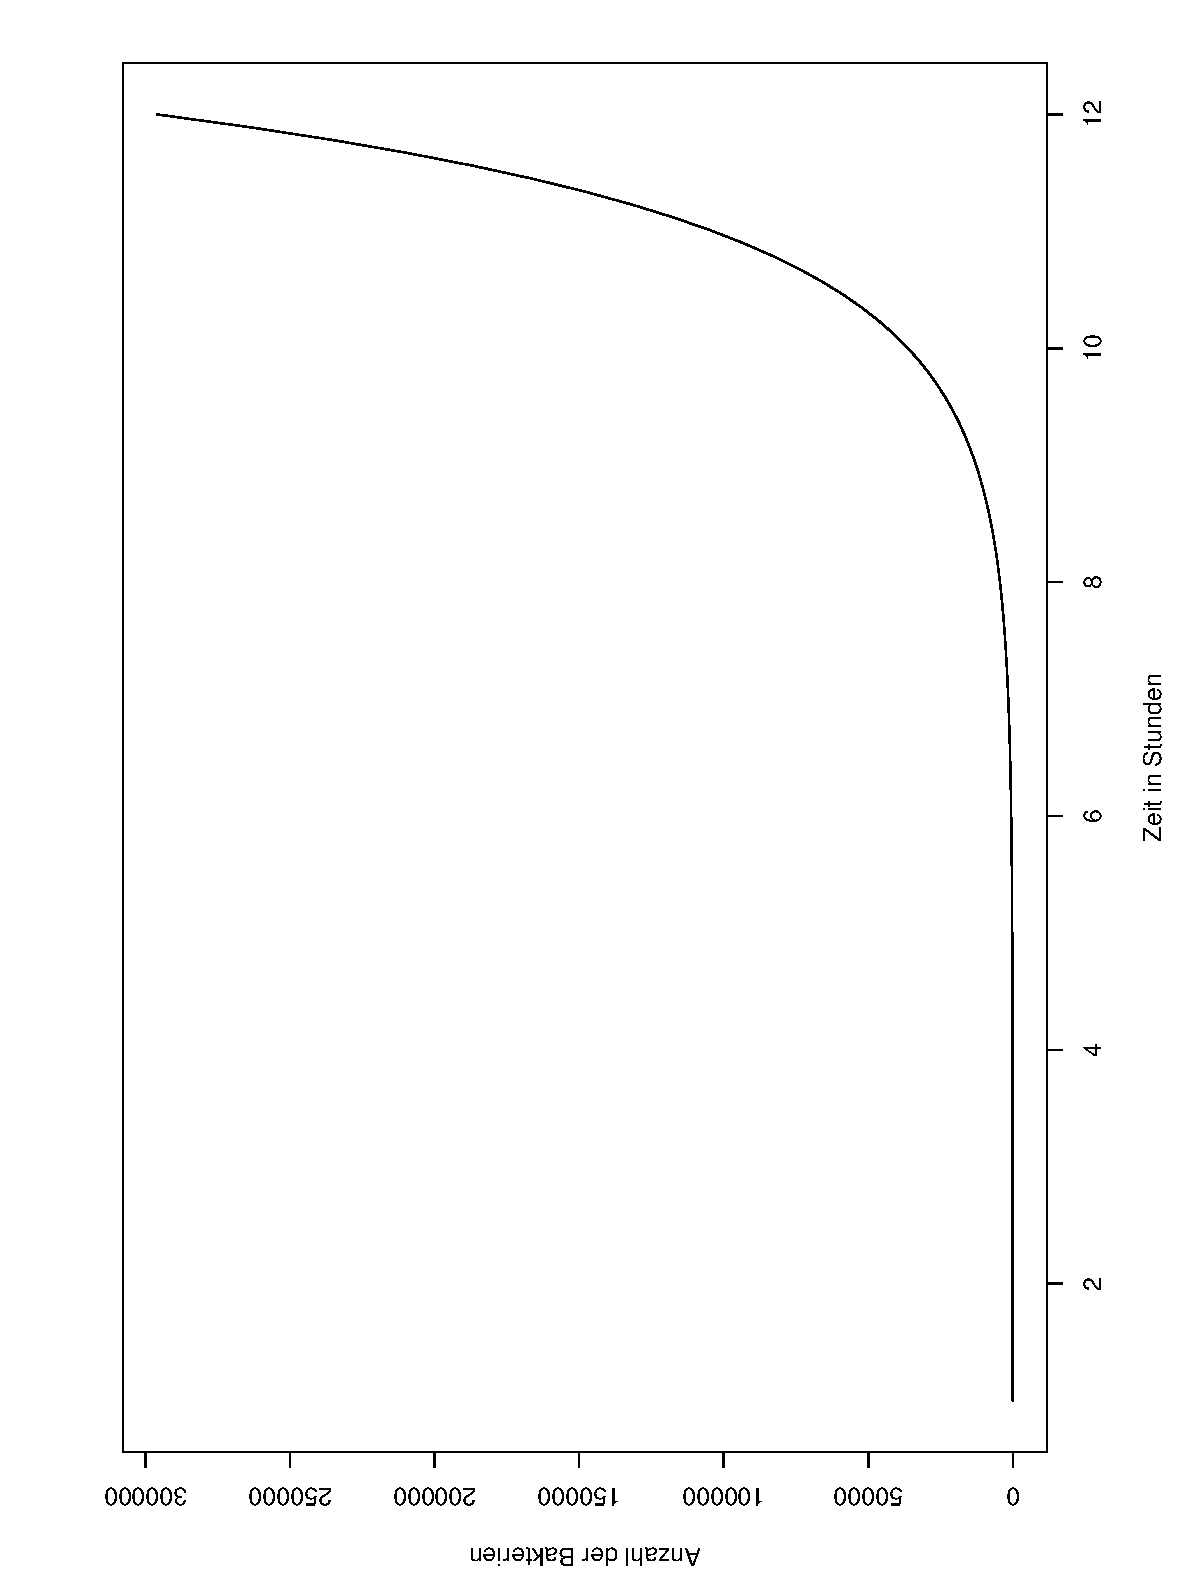
\includegraphics[scale=0.5]{./pictures/ecoli_plot.pdf}		% TODO:schoener machen :\
		\end{center}
		\caption{\slshape{Wachstum von E. coli}}
		\label{fig:ecoliplot}
		\end{figure}

	\item Die einfachste Methode zur Messung des Wachstums ist die Trübungsmessung. Würden Sie diese Methode anwenden, wenn Sie mit \emph{Streptomyceten} arbeiten? Begründen Sie Ihre Antwort!
		Da \emph{Streptomyceten} nicht dispers wachsen,
		ist die Messung des Wachstums mit Trübung	nicht möglich.

		Bei der Trübmessung wird gemessen wieviel des auf die Kultur eingestrahlten Lichtes diese durchdringt.
		Durch zunehmmende Zellzahlen nimmt der Anteil des durch die Kultur Absorbierten Lichtes ab.
		Um diese Methode anwenden zukönnen,
		müssen die Mikroorganismen jedoch dispers wachsen.
		Das heisst keine Zusammenhängenden Strukturen ausbilden. % Todo - Brock überprüfen

	\item Die Proteine FtsZ und MreB sind für die Zellteilung sehr wichtig. Wozu würde die Zerstörung dieser beiden Gene in \emph{E. coli} führen?
		Das Protein \emph{FtsZ}, ``Filamentus temperatur sensitive mutant Z'',
		ist entscheidenen am Prozess der Zellteilung beteiligt.
		Nach der Elongation der Zelle,
		bilden \emph{FtsZ}-Proteine das sogenannte Divisom und,
		trennen die Zelle in zwei Hälften.
		Dabei interagiert der \emph{FtsZ}-Ring mit den bereits duplizierten Nukleoid.
		Entlang des Ringes wird schließlich die neue Zellwand gebildet.
		Diese ist beim Abschnüren der entstehenden Tochterzellen bereits gebilder,
		um die strukturelle Integrität der Zellen zu erhalten.	% todo -pics

		\begin{figure}
		\centering
		\subfloat[FstZ]{\label{fig:fstz}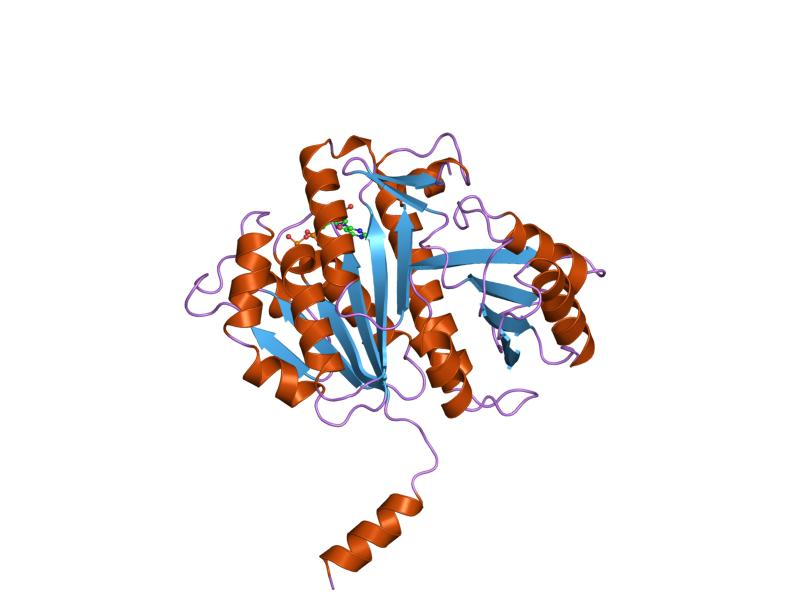
\includegraphics[width=0.44\textwidth]{./pictures/ftsz_800}}
		\subfloat[MreB]{\label{fig:mreb}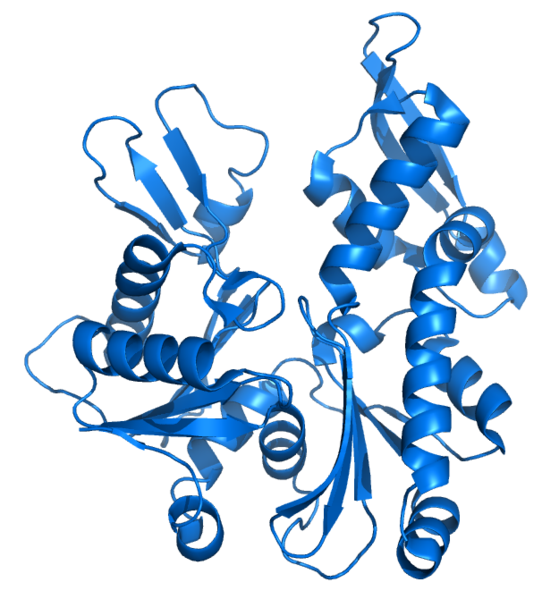
\includegraphics[width=0.25\textwidth]{./pictures/MreB_500}}
		\subfloat[Actin]{\label{fig:fstz}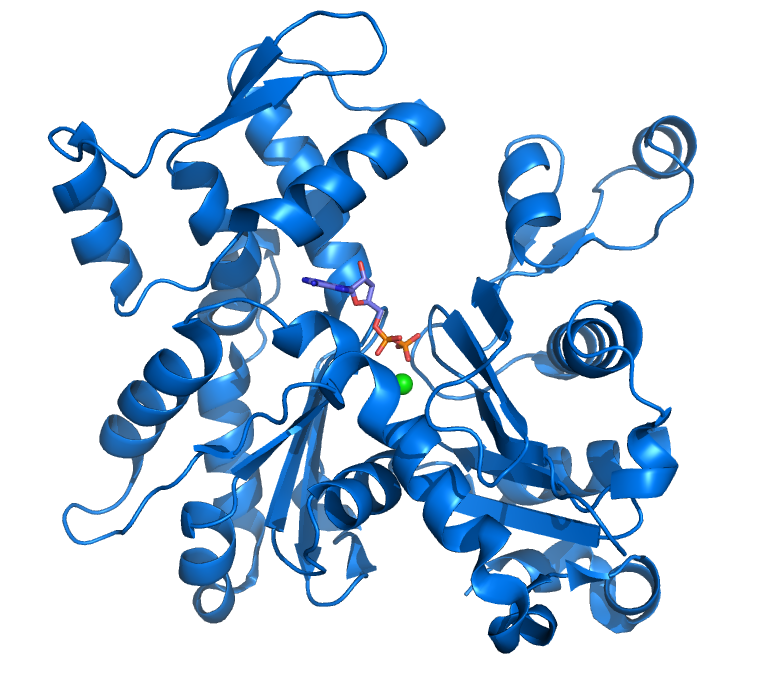
\includegraphics[width=0.3\textwidth]{./pictures/actin_762}}
		\caption{\slshape{Tertiärstruktur von Proteinen mit hoher Beduetung für die Zellteilung und Cytoskelett in \emph{E. coli}}}
		\label{fig:ecoli_proteins}
		\end{figure}

		Bei \emph{MreB} handelt es sich um ein dem \emph{Actin} homolgen Protein.
		Diese Proteine sind mit dem Cytoskellete der Zellen assoziert.
		\emph{MreB} bilder spiralige Bänder innerhalb der cytoplasmatischen Membran.
		In kokkenförmigen Bakterien ist \emph{MreB} nicht gefunden worden.
		Erst durch dieses Protein können Vibrionen, Stäbchen und Spirillen endstehen.
		Bakterien mit einem Mutanten sind jedoch kokkoid.

		Die Tertiärstrukturen der der Proteine sind in Abbildung \ref{fig:ecoli_proteins} dargestellt.
		
	\item Bei steigender Temperatur steigt die Wachstumsrate von Bakterien bis zum Optimum langsam an, dann fällt Sie schnell ab. Begründen Sie diesen Kurvenverlauf!

		Die Enzymatische Aktivität steigt stetig bedingt durch RGT-Regel.
		Übersteigt die Temperatur jedoch eine bestimmte,
		für jeden Mikroorganismus spezifische,
		Schwelle, denaturieren wichtige Proteine.
		Da diese nun nichtmehr ihrer Funktion erfüllen,
		können sich die Mikroorganismen nicht weiter vermehren.
		Zusätzlich wird ab einer spezifischen Temperatur die Membran instabil.

		Die Temperatur darf aber auch eine spezifische Temperatur nicht unterschreiten.
		Bei niedrigen Temperaturen verliert die Membran ihre Fluidität und
		Transportprozesse laufen zu langsam ab so das die Zellen nicht wachsen können.
		Die Minimal-, Optimal- und Maximal-Temperatur werden auch als Kardinaltemperaturen
		bezeichnet und sind in Tabelle \ref{tab:ecolikardinal} für \emph{E. coli} aufgeführt.

		\begin{table}[h!]
		\begin{center}
		\begin{tabular}{l l l} 
		\toprule
		Kardinaltemperatur	&	Wert	&	Begrenzender Faktor\\
		\midrule
		Minimaltemperatur		&	8\textdegree C	&	Membranzustand, RNA \\
		Optimaltemperatur		&	39\textdegree C	&	Optimale Bedingungnen	\\
		Maximaltemperatur		&	48\textdegree C	&	Inaktivierung wichtiger Proteine \\
		\bottomrule
		\end{tabular}
		\caption{Kardinaltemperaturen von \emph{E. coli}}
		\label{tab:ecolikardinal}
		\end{center}
		\end{table}

	\item Warum die Anpassung an niedrige Temperaturen bei Lipiden besonders wichtig? Nennen Sie einige Möglichkeiten dafür!

		Lipide befinden sich in Zellen hauptsächlich in der Membran.
		Durch Kälte sinkt die Fluidität der Membran und sie wird gelartig,
		was die Lebensvorgänge der Mikrooorganismen stark beeinträchtigt.
		Durch eingelagerte Stoffe wie Cholesterin bliebt die Membran fluide.
		Zusäzlich haben an Kälte angepasst Mikroorganismen einen höheren Anteil an ungesättigten Fettsäuren
		in der Membran.
\end{enumerate}

\newpage
\sectionmark{Wachstum der Bakterien II}

\section{Wachstum der Bakterien II}
\label{sec:wachstum2}
\begin{enumerate}
	\item Viele Archaea leben bei extrem hohen Temperaturen, bei denen der DNS-Doppelstrang schmilzt. Haben diese Organismen eine einzel- oder doppelsträngige DNS? Wenn sie doppelsrtängig ist, wie wird erreicht, dass die Stränge nicht auseinanderfallen?
		\label{item:htarchaea}
		Hyperthermophile Archaeen besitzen spezielle Anpassung an extrem hohe Temperaturen.
		Zu dieses speziellen Anpassung zählt ein geringe GC-Gehalt des Genoms,
		da diese Bindung weniger stabil ist.
		Die DNS ist weiterhin mit Proteinen assoziert,
		dies können z.B. Histone sein.
		Durch positives Supercoiling wird die DNS besser vor Temperatureinflüssen geschützt.
		Die reverse Gyrase, welche für diesen Vorgang benötigt wird,
		ist das einzige für hyperthermophile Bakterien und Archaeen spezifische Protein.
		Die Erhöhung der intrazellulären Salzkonzentration verhindert ebenso DNS-Schäden.

		Weiter Anapssungen an hohe Temperaturen umfassen vorallem die Membranen.
		So werden zum Teil die Esterbindungen zwischen Glycerol und den Seitenketten durch Etherbindungen ersetzt.
		Dadurch ergeben sich weniger Doppelbindungen,
		was siche postiv auf die Stabilität der Membran auswirkt.
		Bei eingen Arten wird die Lipid-Doppelschicht durch einen Biphyntanyl-Monolayer erstzt.

		Als Beispiel für ein hyperthermophilen Mikroorganismus ist hier \emph{Pyrolobus fumarii} aufgeführt.
		In Tabelle \ref{tab:pfumariikardinal} sind sine Kardinaltemperaturen aufgeführt 
		(Vergleiche: Tabelle \ref{tab:ecolikardinal}, ``Kardinaltemperaturen von \emph{E. coli}).

		\begin{table}[h]
		\begin{center}
		\begin{tabular}{l r}
		\toprule
		Kardinaltemperatur	&	Wert	\\
		\midrule
		Minimaltemperatur		&	90\textdegree C		\\
		Optimaltemperatur		&	106\textdegree C	\\
		Maximaltemperatur		&	113\textdegree C	\\
		\bottomrule
		\end{tabular}
		\caption{Kardinaltemperaturen von \emph{Pyrolobus fumarii}}
		\label{tab:pfumariikardinal}
		\end{center}
		\end{table}

	\item Warum ist \emph{Prochlorococcus marinus} von so großer Bedeutung? Wo leben diese Bakterien?

		\emph{P. marinus} ist wohl der häufigst und am weitesten verbreitet Organismus der Welt.
		Weiterhin gehört es zu den kleinsten bekannten Cyanobakterien, 
		und lebt in den Ozeanen von 40\textdegree Nord bis 40\textdegree Süd in Meerestiefen von 100 bis 200m.
		Durch die Konzentration von 10\textsuperscript{4} bis 10\textsuperscript{5} Zellen pro ml Meerwasser,
		ist er wahrscheinlich der wichtigste Primäproduzent im Ozean.
		Einzelne Zellen von \emph{P. marinus} haben einen Durchmesser von 0,5 bis 0,8 \begin{math}\mu m\end{math}.

	\item Welche Anpassungen weisen die Lipide von hyperthermophilen Organismen auf?

		Siehe Frage \ref{sec:wachstum2}.\ref{item:htparchaea}.

	\item Welche Bakteriengruppen spielen in der Darmflora eine besonders wichtige Rolle?
		
		In Tabelle \ref{tab:darmMO} befindet eine Übersicht über das Microbiom im menschlichen Darm.

		\begin{table}[h]
		\begin{center}
		\begin{tabular}{l l}
		\toprule
		Domäne		&		Verbreitung \\
		\midrule
		Archaea		&		\emph{Methanobervibacterium smithii}	\\
		Eukarya		&		wenige Pilze und Hefen 		\\
		Bacteria		&		Vertreter aus 9 Phyla, circa 1000 Arten 	\\
		Phagen		&		1200 virale Genotypen, meist Phagen von Firmicuten \\
		\bottomrule
		\end{tabular}
		\caption{Übersicht über (bekannte) Mikroorganismen im menschlichen Darm}
		\label{tab:darmMO}
		\end{center}
		\end{table}

		Die Darmflora setzt sich zum 99\% aus den bakteriellen Gruppen \emph{Firmicutes},
		\emph{Bacteroidetes}, \emph{Proteobacteria} und \emph{Actinobacteria} zusammen.		% cc-sa by de.wikipedia.org/wiki/Darmflora

	\item Welche Leistung erbringt die Darmflora für den Menschen?
		
		Die Darmflora erbringt zahlreiche Leistungen für den Menschen.
		Durch die starke Integration und Interaktion der Mikroorganismen mit dem Menschen,
		wir dieser auch als ``Superorganismus'' bezeichnet.

		\begin{description}
		\item[Häufige Gene im Microbiom] \hfill \\
			Depolymerasen im Kohlenstoff-Stoffwechsel
		\item[Nahrungskette] \hfill
			\begin{itemize}
			\item Auf - und Abbau von Nahrung: \\
			Polysaccharide \textrightarrow Karbonsäuren \textrightarrow Gase
			\item Methanbildung zur Entfernung von Wasserstoff
			\end{itemize}
		\item[Organische Säuren] \hfill \\
			Aufnahme durch den Wirt - bis zu 10\% der Kalorienaufnahme des Wirtes	
		\end{description}

		Die Zusammensetzung des Mikrobioms ist abhängig von der Ernährung des Menschen.
		Schlanke Menschen haben einen erhöhten Anteil von bis zu 20\% \emph{Bacteroides},
		wohingengen Vollschlanke eine höheren Anteil an \emph{Firmicutes} im Microbiom haben.
		Jedoch ist die Zusammensetzung des Microbioms eine folge des Köpergewichtes,
		nicht umgekehrt.

\end{enumerate}

\newpage
\sectionmark{Biotechnologie I}

\section{Biotechnologie I}
\begin{enumerate}
	\item Nennen Sie Beispiele biotechnologisch hergestellter Produkte?
	\item Was ist der Pasteur-Effekt?
	\item Wie ausgeprägt ist der Pasteur-Effekt bei Saccharomyces cerevisiae und welche
	\item Bedeutung hat dies für biotechnologische Anwendung?
	\item Was ist der Unterschied zwischen ober- und untergärigen Hefen in Bezug auf die Bierproduktion?
	\item Wie wird Bier hergestellt?
	\item Welche Stoffwechselwege werden für die biotechnologische Produktion von Ethanol genutzt?
	\item Welche Organismen können 1,3-Propandiol produzieren?
	\item Wie wird Sauerkraut hergestellt?
	\item Wie wird Joghurt hergestellt?
	\item Welche Möglichkeiten gibt, um einen Stamm für einen biotechnologischen Prozess zu verbessern?
\end{enumerate}

\newpage
\sectionmark{Biotechnologie II}

\section{Biotechnologie II}
\begin{enumerate}
	\item Wie unterscheiden sich unvollständige Oxidationen von Biotransformationen (Biokonversionen)?
		
		Bei der vollständigen Oxidation wird Sauerstoff komplett zu \ce{CO2} oxidiert.
		Eine unvollständige Oxidattion ist gegeben wenn,
		wenn der Sauerstoff nicht vollständig oxidiert wird,
		sondern das ein Zwischenprodukt das Ziel der Oxidation ist.
		Unvollständige Oxidationen sind meist mit Wachstumsvorgängen assoziert.
		
		Bei einer Biokonversion handelt es sich um einen Co-Metabolismus,
		welche in einer stationären Phase (also nicht während des Wachstums) stattfinden.
		
	\item Nennen sie biotechnologisch relevante Produkte die auf unvollständigen mikrobiellen Oxidationen beruhen.
		
		\begin{itemize}
			\item Acetat
			\item Gluconat
			\item Fumarat
			\item Citrat und andere organische Säuren
			\item Aminosäuren
			\item Alkohole
		\end{itemize}
		
	\item Nennen Sie Charakteristika der Essigsäurebakterien Gluconobacter und Acetobacter.
	
		\begin{itemize}
			\item Gram-negativ
			\item bewegliche Stäbchen
			\item aerob
			\item unvollständige Oxidation von Alkoholen und Glucose
		\end{itemize}
			
	\item Was unterscheidet die Unteroxidierer (Suboxidanten) von den Überoxidierern (Peroxidanten)? Nennen sie typische Vertreter beider Gruppen.
	
		\begin{description}
			\item[Peroxidanten] \hfill \\
				Die gebildeten organischen Säuren werden nach dem Verbrauch des Substrats vollständig oxidiert.
				Sie besitzen meist einen vollständigen Tricarbonsäurezyklus (z.B. \emph{Acetobacter}).
			\item[Suboxidanten] \hfill \\
				Die gebildeten organischen Säuren werden nicht verbraucht.
				Sie besitzen keinen Vollständigen Tricarbonsäurezyklus (z.B. \emph{Gulconobacter}).
		\end{description}
		% TCA == Citratzyklus?!
		
	\item Benennen sie die enzymatischen Schritte für die Umsetzung von Ethanol zu Acetat durch Essigsäurebakterien.
	\item Durch welche Verfahren wird Essig hergestellt?
	\item Welche Rolle spielen Essigsäurebakterien bei der Synthese von Ascorbinsäure?
	\item Nennen sie Beispiele für durch Stress-induzierte unvollständige Oxidationen.
	\item Unter welchen Bedingungen produziert \emph{Aspergillus niger} Citrat?
	\item Was begünstigt die Glutamat-Ausscheidung von \emph{Corynebacterium glutamicum}?
	\item Für welche Anwendungsbereiche ist die biotechnologische Produktion von Aminosäuren bedeutsam?
	\item Wie unterscheiden sich unvollständige Oxidationen und Sekundärstoffwechsel voneinander?
	\item Was versteht man unter Tropo- und Idiophase?
	\item Nennen Sie Beispiele für den Wirkort von Antibiotika.
	\item Welche Organismen können Vitamin B12 synthetisieren?
	\item Wie ist ein Metagenom definiert?
	\item Nennen sie zwei grundsätzliche Vorgehensweisen zur Gewinnung von neuen Genen und Biokatalysatoren aus Metagenomen mir Beispielen?
\end{enumerate}

\newpage
\sectionmark{Infektionsbiologie}

\section{Infektionsbiologie}
\begin{enumerate}
	\item Nennen Sie mindestens fünf bakterielle Krankheitserreger, die von ihnen verursachten Krankheiten und die systematischen Gruppen, zu denen diese Bakterien gehören!
	\item Nennen Sie einige typische Mikroorganismen, die den menschlichen Organismus normalerweise besiedeln und die dazugehörigen Organe und typischen Lebensbedingungen!
	\item Warum ist Saccharose hochgradig kariogen, Fructose aber nicht? Welche Bakterien spielen bei der Karies eine wichtige Rolle?
	\item Was sind die wichtigsten Schritte bei der Etablierung einer Infektion? Nennen Sie einige Faktoren, die den Bakterien dabei helfen!
\end{enumerate}

\newpage
\sectionmark{Stoffkreisläufe}

\section{Stoffkreisläufe}
\begin{enumerate}
	\item Nennen sie dissimilatorische Prozesse im Stickstoff-Kreislauf?
		
		\begin{itemize}
			\item Anaerobe Denitrifikation \hfill \ce{NO3-} \textrightarrow \ce{NO2-} \textrightarrow \ce{N2}
			\item Aerobe Denitrifikation \hfill \ce{NO4+} \textrightarrow \ce{NO2-} \textrightarrow \ce{NO3-}
			\item Anammox \hfill \ce{NO2-},\ce{NH4+} \textrightarrow \ce{N2}
			\item Assimilation \hfill \ce{NH4+} \textrightarrow \ce{NH3}
		\end{itemize}

	\item Welche Rolle spielen Denitrifikanten und Nitrifikanten bei der Abwasserbehandlung in Kläranlagen?

		Durch Denitrifikation geschieht die Stickstoff-Eleminierung.
		Dies kann auch durch das Anammox-Verfahren geschehen,
		bei dem jedoch weniger Biomasse endsteht.

		Bei der Denitrifikation wir zunächst aerob \ce{NH4+} in \ce{N03-} unter \ce{o2}-Gabe umgesetzt.
		Dann wird das \ce{NO3-} mit organimschem Kohlenstoff,
		beispielsweise aus Methanol,
		in Stickstoffgas und Biomase umgesetzt.

		Beim Aanmmox-Verfharen wird  die Hälfte des \ce{NH4+} mit \ce{O2} in\ce{NO2-} umgestetzt.
		Dieses wird zusammen mit dem restlichen \ce{NH4+} in Stickstoffgas und wenig Biomase umgesetzt.

	\item Welche Umsetzung katalysieren Anammox-Bakterien?
	\item Nennen Sie \ce{N2}-Fixierer!
	\item Können eukaryontische Organismen \ce{N2} fixieren?
	\item Wie ist Nitrogenase aufgebaut?
	\item Beschreiben Sie den Ablauf der \ce{N2}-Reduktion an der Nitrogenase!
	\item Wie kann die Nitrogenase vor dem Kontakt mit Sauerstoff geschützt werden?
	\item Welche Rolle spielen phototrophe Bakterien im Schwefel-Kreislauf?
	\item An welchen Schritten im Stickstoff- und Schwefel-Kreislauf sind chemolithoautotrophe Organismen beteiligt (Nennen sie Namen für typische Vertreter)?
	\item Welche Organismengruppen können für Gebäudeschäden verantwortlich sein und warum?
	\item Welche Rolle spielen Sulfatreduzierer im Schwefel-Kreislauf?
\end{enumerate}

\newpage
\sectionmark{Systematik der Mikroorganismen}

\section{Systematik der Mikroorganismen}
\subsection{Einführung}
\begin{enumerate}
\item Warum ist die ribosomale RNA so gut als Marker für die Untersuchung von Verwandtschaftsverhältnissen geeignet?
	
	Die 16S rRNA ist universell in allen bekannten zellulären Organismen verbreitet
	und erfüllt auch in allen dür die gleich Funktionalität verantwortlich.
	Weiterhin lässt sie sich gut isolieren
	und durch Alignemnts lassen sich die Sequenzen verschiedener Organismen sehr gut vergleichen.
	Durch die geringe gesamte Mutationsrate lassen sich gut entfernte Verwandschaften nachweisen.
	Mit einer Analyse von variablen Bereichen ist auch die Untersuchung von näher verwandten Arten gut möglich.

\item Wie geht man bei der Beschreibung eines neuen Organismus vor?
	
	Detaillierte Beschreibung von:
	\begin{itemize}
		\item Physiologische Eigenschaften (Größe, Gram-färbung, Geißel, Form, etc.)
		\item Temperaturbereich
		\item Habitat
		\item Metabolismus
		\item Genetische Eigenschafte (GC-Gehalt, Proteinfunktionen, Plasmide)
	\end{itemize}

	Weiterhin muss ein Typstamm hinterlegt werden,
	der von anderen Froschern angefordert werden kann.

\end{enumerate}

\subsection{Archaea}
\begin{enumerate}
	\item Vergleichen Sie wichtige molekularbiologische und physiologische Eigenschaften der drei Organismenreiche!
		
		In Tabelle \ref{tab:domaenenuberblick} ist eine Übersich über die Eigenschaften der drei Organismenreiche.	

		\begin{table}[h!]
		\begin{center}
		\begin{tabular}{l l l l} 
		\toprule
		Merkmal		&	Bacteria		&	 Archaea				&	 Eukaraya		\\
		\midrule
		Zellkern 	&	nein			&	 nein					&	 ja		\\
		cccDNA		&	ja				&	 ja					&	 nein (linear)			\\
		Histone		&	nein			&	 ja					&	 ja		\\
		Zellwand		&	Murein		&	 kein Murein		&	 kein Murein		\\
		Membranlipid&	Ester			&	 Ether				&	 Ester		\\
		\midrule
		Ribosomen	&	70S			&	 70S					&	 80S		\\
		Ini-tRNA		&	f-Met			&	 Met					&	 Met		\\
		Introns 		&	nein			&	 nein					&	 ja		\\
		ja				&	Operon		&	 ns					&	 nein		\\
		Cap/poly-A 	&	nein			&	 nein					&	 ja		\\
		Plasmide		&	ja				&	 ja					&	 selten		\\
		RNA-Pol			&	ne (4 UE)	&	 viele (8-12 UE)	&	drei (12-14 UE)	\\
		TK-Faktoren		&	nicht nötig	&	 benötigt			&	benötigt		\\
		Promotoren		&	-10, -35		&	 TATA					&	TATA		\\
		\midrule
		Methanbildung		&	nein			&	 ja					&	nein		\\
		S-Reduktion		&	ja				&	 ja					&	nein		\\
		Nitrifizierung	&	ja				&	 nein					&	nein		\\
		Denitrifizierung		&	ja				&	 ja					&	nein		\\
		N-Fixierung		&	ja				&	 ja					&	nein		\\
		Photosynthese		&	ja				&	 nein					&	nein (Plastiden)	\\
		Lithotrophie	&	ja				&	 ja					&	nein		\\
		Grw. > 80°C		&	ja				&	 ja					&	nein		\\
		\bottomrule
		\end{tabular}
		\caption{Übersicht über die Eigenschaften der drei Organismenreiche.}
		\label{tab:domaenenuberblick}
		\end{center}
		\end{table}

	\item Nennen Sie zwei wichtige Gruppen der Euryarchaeota! Wo würden Sie diese Organismen suchen?
		
		\begin{description}
			\item[Pyrococcus] \hfill \\
				An heißen Standorten.
				(Taq-Polymerase, PCR ?)
			\item[Methanogene Euryarchaeota] \hfill \\
				Die Methanbildenden Euryachaeota, 
				die Gruppen \emph{Methanobacterium}, \emph{Methanococcus} und \emph{Methanosarcina},
				bilden Methan in den Biogas-Anlagen von Klärwerken.
		\end{description}
		Insgesamt lassens ich die Euryarchaeota als eine Gruppe von Extremophilen beschreiben.

	\item Wiederholen Sie kurz die wichtigsten Schritte der Methanbildung! Welche Rolle spielen ungewöhnliche Koenzyme bei diesem Stoffwechselweg?

		Siehe Anaerobe Atmung?!
	
	\item Wie schützt Thermoplasma seine Membran vor der hohen Temperatur?

		Thermoplasma besitzt keine Zellwand sondern eine einzigartige Zellmembran.
		Diese besteht aus Tetraether-Lipiden mit Glukose- und Mannoseeinheiten.

	\item Bei der PCR werden DNA-Fragmente zunächst bei 96\textdegree C aufgeschmolzen. Einige Archaea leben bei wesentlich höheren Temperaturen. Daher gibt es zwei Möglichkeiten für deren DNA:
	\begin{enumerate}
		\item Sie haben einzelsträngige DNA. Wie könnte in diesem Fall die Replikation ablaufen?
				
			Die DNA könnte von einer modifizierten RNA-Polymerase abgelesen werden.

		\item Sie haben doppelsträngige DNA. Wie kann der Doppelstrang bei so hohen Temperaturen stabil sein? Entscheiden Sie sich für eine der Möglichkeiten und beantworten Sie die Zusatzfrage!
			
			Die DNA könnte stark verpackt sein und durch einen hohen GC-Gehalt an die hohhen Temperaturen angepasst sein.

	\end{enumerate}
\end{enumerate}
	
\subsection{Bakterien}
\begin{enumerate}
	\item \emph{Deinococcus radiodurans} kann sehr hohe Strahlendosen überleben. Welche Mechanismen helfen diesem Bakterium dabei?
		
		\emph{Deinococcus radiodurans} enthält viele Karotinoide,
		was auch die rote Färbung bedingt.
		Die Ursachen der hohen Resistenz liegt in den sehr effizienten DNA-Reparatursystemen.
		Dieses beinhaltet verschiedene Enzyme für verschiedene Schäden,
		welche selbst in der Lage sind fragmentierte DNA wieder zu verbinden.

	\item Zeichnen Sie schematisch den Aufbau einer Spirochaeten-Zelle auf (Längsansicht und Querschnitt). Erklären Sie die wichtigsten Komponenten!
		
		\begin{figure}[ht!]
		\begin{center}
		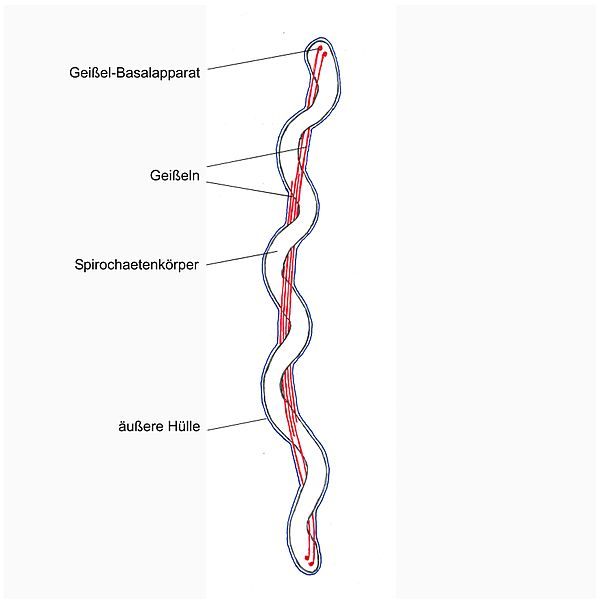
\includegraphics[scale=0.42]{./pictures/schema_spiro_596}
		\end{center}
		\caption{\slshape{Grobes Schema einer Spirochaetenzelle}}
		\label{fig:spiroschema}
		\end{figure}
			
	\item Erläutern Sie den Lebenszyklus der Chlamydien! Warum sind diese Bakterien (\emph{C. trachomatis}) als Krankheitserreger so bedeutsam?
		
		Chlamydien sind obligate intrazelluäre Parasiten.
		Sie reduzieren die Stoffwechselleistung der Zellen und werden deshalb auch als ``Energieparasiten'' bezeichnet.
		Chlamydien können in zwei Formen auftreten.
		Der sogenannten ``Elementary body'' kommt außerhalb von Zellen vor und dringt
		durch Phagocytose in die Wirtzelle ein.
		Nun wandelt er sich zum sogenannten ``Reticulate body'',
		der zweiten Form der Chlamydien,
		und vermehert sich.
		Nach dem genug ``Reticulate bodies'' endstanden sind,
		wandeln sich diese wieder in ``Elementary bodies'' um und verlassen den Wirt um andere Zellen zu besiedeln.

		Chlamydien Infektionen bleiben oft unendekt,
		da sie symptomlos verlaufen.
		So können sich die Bakterien im Uro-Genitaltrakt einnisten
		und Unfruchtbarkeit auslösen.
		Im Auge kann \emph{C. trachomatis} ein Infektion auslösen die zur Erblindung führt.

	\item Die Cyanobakterien sind eine extrem erfolgreiche Bakteriengruppe: Sie leben nicht gerade von Luft und Liebe, aber trotzdem von sehr einfachen Verbindungen. Nennen Sie C-Quelle, N-Quelle, Elektronendonor und Energiequelle dieser Bakterien!
		\begin{description}
			\item[C-Quelle]	\ce{CO2}, Glukose
			\item[N-Quelle]	Nitrate, Ammonium, \ce{N2}-Fixierung
			\item[Elektronendonor] 	Wasser (oxygene Photosynthese)
			\item[Energiequelle]		Licht
		\end{description}

	\item Glauben Sie, dass ein solch vielfältiges Leben, wie wir es auf der Erde kennen, möglich wäre, wenn es die oxygene Photosynthese nicht geben würde?

		Nein. Aber ich sollte das in der Bibel nachlesen.

	\item Cyanobakterien und -Proteobakterien können leicht mit eukaryontischen Zellen interagieren. Nennen Sie ein paar Beispiele für solche Interaktionen (mindestens sechs)!
	
		\begin{itemize}
			\item Plastiden \hfill (Chloroplasten, Rhodoplasten
			\item Symbiosen \hfill (Lebermoose, Cycadeen, Farnen)
			\item Sybiose mit Anabena - Azolla \hfill (N-Quelle für Reis)
			\item phototophe Komponente von Flechten
		\end{itemize}

	\item Was sind die Schritte, einen künstlichen Organismus herrzustellen? Halten Sie das für eine gute Idee?

		\begin{itemize}
			\item Minimales Gensets ermitteln
			\item Assemblierung des künstlichen Minimalgenoms aus Oligonukleotiden
			\item Assemblierung zu Chromosomen
			\item Einführen des künstlichen Genoms in ein Zelle deren DNA zuvor entfernt wurde
		\end{itemize}

	\item Milchsäurebakterien spielen für viele biotechnologische Vorgänge in der Nahrungsmittelindustrie eine große Rolle. Was unterscheidet homo- und heterofermentative Milchsäurebakterien? Sie erhalten die Aufgabe, ein heterofermentatives Bakterium in ein homofermentatives zu verwandeln. Wie gehen Sie vor?

		Bei der homofermentativen Milchsäuregärung wird die Glykolyse anders durchgeführt.
		Da bei heterofermentativen Milchsäure gäreren die Aldolase fehlt,
		verwenden sie den Pentosephosphat-Weg.
		Deshalb endsteht bei ihnen als Endprodukt zusätzlich Ethanol.

	\item Streptomyceten sind wichtige Antibiotikabildner. Nennen Sie einige von Streptomyceten gebildete Antibiotika und die Erreger, die man damit bekämpfen kann. Warum sterben eigentlich die Streptomyceten nicht selbst an den von ihnen gebildeten Antibiotika?

		In Tabelle \ref{tab:strpetoantibiose} befindet sich ein Übersicht über die von Streptomyceten gebildeten Antiobiotika.
		
		\begin{table}[h!]
		\begin{center}
		\begin{tabular}{l l l l} 
		\toprule
		Gruppe			&	Name				&	Produzent			& 	wirksam gegen	\\
		\midrule
		Aminoglcycine	&	Streptomycin	&	S. griseus			&	Gram-negative		\\
		\multirow{2}{*}&	Spectinomycin	&	S. spp.				&	M. tuberculosis		\\
							&	Neomycin			&	S. fradiae			&	Breitband		\\
		Tetracycline	&	Tetracyclin		&	S. aureofaciens	&	Breitband		\\
		Macrolide   	&	Erythromycin	&	S. erythreus		&	meiste Gram-positive		\\
		Polyene     	&	Nystatin			&	S. noursei			&	Pilze		\\
		keine       	&	Chloramphenicol&	S. venezuelae		&	Breitband		\\
		\bottomrule
		\end{tabular}
		\caption{Übersicht über die Antibiotika Produczenten der \emph{Streptomyceten}.}
		\label{tab:strpetoantibiose}
		\end{center}
		\end{table}

		Durch Verschiedene Mechanismen können sich die Strptomyceten vor ihren eigenen Antibiosen schützen.
		Durch Methylierung der eigenen rRNA geht der zum Beispiel der Angriffsort verloren.
		Dies geschieht auch durch veränderung der nicht ribosomalen Ziele,
		wie der DNA-Gyrase, der RNA-Polymerase und EF-Tu. %das gehoert zu tRNA und bindet AS im 50S ribosom o0
		Weiterhin werden die Inhibitoren der Translation durch Phosphorylierung,
		Acetylierung und Glykoylierung modifiziert.

	\item Wofür steht das E. in \emph{E. coli}? 

		Escherichia.
		%bam!

	\item Ralstonia eutropha wurde in Weende entdeckt. Welche Eigenscaften machen dieses Bakterium so interessant?
		
		Das Bakterium ist in der Lage Polyhydroxybuttersäure.
		Diese kann verwendet werden,
		um Biopolymere zu erzeugen.
		Durch Zugabe von bestimmten Stoffe kann man dann Plastik-artige Materialien erzeugen,
		welche jedoch biologisch abbaubar sind.

	\item Zu den Gamma-Proteobakterien gehören die Enterobakterien. Nennen Sie einige Vertreter dieser Bakteriengruppe!
	
		\begin{itemize}
			\item Legionella pneumophila	\hfill (pathogen)
			\item Vibrio cholerae
			\item Photobacterium
			\item Haemophilus influenzae 	\hfill (pathogen)
			\item Acinetobacter calcoaceticus
			\item	Pseudomonas aeruginosa 	\hfill (pathogen)
			\item Azotobacter vinelandii
			\item	Xylella fastidiosa 	\hfill (pathogen)

		\end{itemize}

		Fakultative Anaerober, die alle sehr nahe miteinander verwandt sind.

	\item Zu den Delta-Proteobakterien gehören die Gattungen Myxococcus, Bdellovibrio und Geobacter. Nennen Sie die wichtigsten Eigenschaften bzw. Charakteristika dieser Bakterien!
		
		\begin{description} 
			\item[Myxococcus] \hfill \\
				Sozial-lebende Proteobacterien, die komplizierte Strukturen ausbilden.
				Sie sind beweglich und machen bei reichem Nährstoffangebot einer schwärmende Bewegung.
				Bie Nährstoffarmut erfolgt ein zusammenziehen und das bilden von Fruchtkörpern aus etwa 10.000 Zellen.
				Ernähren sich auch von anderen Bakterien, beispielsweise \emph{E. coli}.
				Die Fruckkörper können bis zum 1 mm  groß werden.
			\item[Bdellovibrio] \hfill \\
				Lebt parasitär an anderen gram-negativen Bakterien.
				Sie lagern sich ein ins Periplasma,
				in dem nun als Bdelloplasten an und saugen den Wirt aus.
			\item[Geobacter] \hfill \\
				Anaerobe Atmung, mit ungewöhnlichen Elektronenakzeptoren (z.B. Uran).
		\end{description}

\end{enumerate}

\subsection{Viren und Prionen}
\begin{enumerate}
	\item Welche subzellulären Krankheitserreger kennen Sie? Bei welchen Organismengruppen können diese Erreger Krankheiten auslösen?
		
		\begin{itemize}
			\item Viren
			\item Viroide
			\item Prionen
			\item Phagen
		\end{itemize}
		
		In allen Domänen des Lebens gibt es spezielle Viren und Phagen.

	\item In welchen Zustandsformen können Viren und Phagen nach der Infektion in der Zelle vorliegen!

		\begin{description}
			\item[Replikationsaktiver Zustand] \hfill \\
				Eine aktive Replikation der Viren findet statt und es werden Nachkommenvieren gebildet.
				%klingt komisch ist aber so.
			\item[Latenzzustand (Lysogenie)] \hfill \\
				Die Zelle ruht mit dem ins Genom integriertem Virus.
		\end{description}

	\item Welches genetische Material besitzt das HI-Virus? 
		
		ss RNA Retroviren - Verletz das zentrale Dogma der Molekularbiologie!\\
		\vspace{1cm}
		reverse Transcriptase(ss RNA) \textrightarrow ds DNA \ldots

	\item Erläutern Sie kurz den Lebenszyklus des Phagen Lambda!

		Die Phage Lambda kann sich nach der Infektion in einen lysogenen Zyklus
		und einen lytischen Zyklus.
		Wobei letzterer für die Vermeherung und weitere Verbreitung dient.
		Im lysogenen Zyklus wird das Genom der Phage in das Genom des Wirtes eingebaut und kann dort überdaueren.
		Durch UV-Strahlung wird der lytische Zyklus ausgelöst.

	\item Bei der spongiformen Enzephalitis kann eine erblich bedingte Krankheit infektiöse Erreger hervorbringen. Wie ist das möglich?
		
		Gerstmann-sträußler-Sheinker / fCJD ist erblich übertragbar,
		aber alle Prionen erzeugen ein Prionenprotein welches infektiös ist.

\end{enumerate}

\newpage
\sectionmark{Genetik}
\section{Genetik}

\begin{enumerate}
		        \item Wie groß sind bakterielle Genome?
				$580070$ Bp (Mycoplasma Genitalium - $9.6 * 10^6$ (Myxococcus xanthus)
			\item Welche Topologie der DNA wird durch die Gyrase erzeugt?
				Negatives Supercoiling (Entwindung der DNA)
			\item Wie nennt man den Start- bzw. Endpunkt der DNA Verdopplung bei einem bakteriellen Chromosom?
				Origin/Terminus of Replication
			\item Was f\"ur Eigenschaften sind vorwiegend auf Plasmiden kodiert?
				\begin{itemize}
					\item Resistenzeigenschaften (Antibiotikaresistenzen etc..)
					\item Metabolische Eigenschaften 
					\item Wirt-veraendernde Eigenschaften 
					\item Sonstige 
				\end{itemize}
			\item Welche Banden k\"onnen bei einer Agarosegelkontrolle einer Plasmidpr\"aparation auftauchen?
				Genetik.pdf, Seite 10, kack folien.
			\item Welche zwei Enzymtypen werden vom Molekularbiologen f\"ur Klonierungen eingesetzt?
				Restriktionsenzyme
				\begin{itemize}
					\item Klasse I und III: Restritkion und Modifikation in einem Komplex, Erkennen und Schneiden entfernt voneinander
					\item Klasse II: Restriktion getrennt von Modifikation, Erkennen und Schneiden an gleicher Stelle
				\end{itemize}
			\item Wie unterscheiden sich TypI und TypIII Restriktionsenzyme von TypII Enzymen?
				Siehe letzte Frage.
			\item Welche nat\"urlichen Wege gibt es mit denen Mikroorganismen Fremd-DNA aufnehmen k\"onnen?
				\begin{itemize}
						\item Transformation (ohne direkten Zellkontakt), Einstr\"angige DNA wird in Zelle aufgenommen
						\item Konjugation (direkter Zell-Zell-Kontakt), F+ Zelle kann F-Plasmid \"uber Pilus an F- Zelle \"ubertragen.
						\item Transdukton (mittels Phagen)
				\end{itemize}
			\item Welche Eigenschaften hat der EAHEC Erreger per Konjugation und welche durch Transduktion erworben?
				\begin{itemize}
					\item pAA-Plasmid \"uber Konjugation von EAEC
					\item Gen fuer Shiga Toxin durch Transduktion STX-Phage ??
				\end{itemize}

\end{enumerate}



\end{document}
\end{input}
